\documentclass{article}
\usepackage[UTF8]{ctex}
\usepackage{enumitem}
\usepackage{graphicx}
% \usepackage{amsmath}
\usepackage{amsmath,amsfonts}
\usepackage{hyperref}

\begin{document}

\title{基于xxx对洛杉矶犯罪情况的预测}
\author{21311570,21311571}
\date{\today}

\maketitle

\renewcommand{\abstractname}{摘要}  % 更改摘要名称

\begin{abstract}
    本实验旨在通过机器学习方法对洛杉矶的犯罪情况进行预测。我们使用了洛杉矶市历史犯罪数据集(2020-2023),并采用了一种xx算法(例如决策树、随机森林或神经网络)来构建预测模型。我们将数据集划分为训练集和测试集,通过评估模型在测试集上的性能来验证预测模型的准确性。本实验的初衷是为亲爱的洛杉矶居民提供一个赛博算命的方法,预测此时此刻可能会在什么地方遇害,然而训练效果欠佳。
\end{abstract}

\section{引言}
犯罪预测是应用机器学习和数据分析的一个重要领域。通过分析历史犯罪数据,我们可以识别出与犯罪相关的模式和趋势,并利用这些信息来预测未来可能发生的犯罪事件。这种预测能力可以帮助居民避免潜在的危险,保护自身安全。

\section{数据预处理}

\begin{figure}
    \centering
    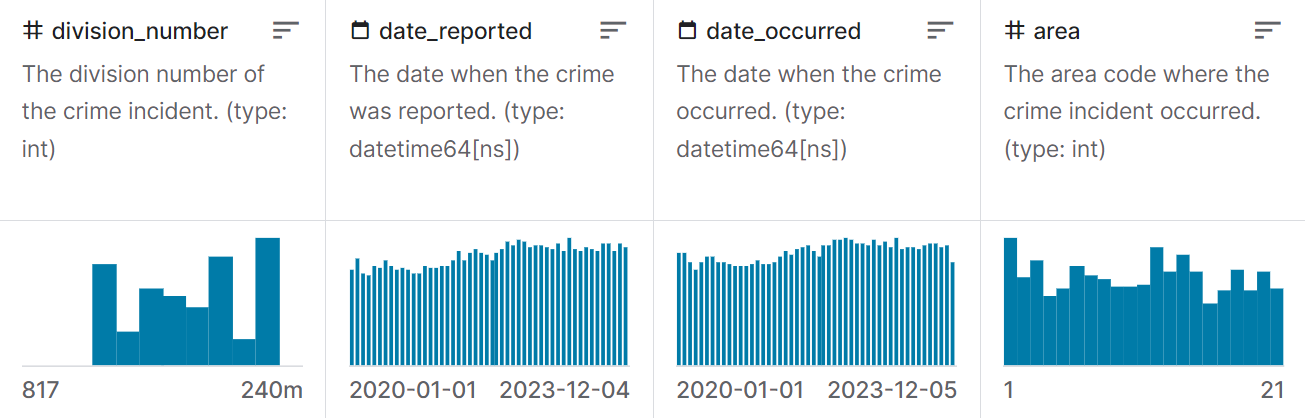
\includegraphics[width=1\textwidth]{../pic/Screenshot 2024-01-12 111029.png}
    \caption{Details of the dataset}
    \label{fig:Details}
\end{figure}


我们使用的数据集\href{https://www.kaggle.com/datasets/asaniczka/crimes-in-los-angeles-2020-2023/data}{Los Angeles Crime Data 2020-2023}来自Kaggle\footnote{Kaggle:一个数据科学竞赛和社区平台。该平台提供了丰富的数据集供研究和分析使用。\\\url{https://www.kaggle.com/}}。该数据集包含了多个属性,包括division\textunderscore{}number(犯罪事件的分区编号)、date\textunderscore{}reported(报告犯罪的日期)、date\textunderscore{}occurred(犯罪发生的日期)、area(犯罪事件发生地的区号)等27个属性。在预处理阶段,我们对数据进行了清洗和转换。这包括处理缺失值、转换日期和时间格式、对分类属性进行编码等(这些好像都是后面的)。

\section{特征选择}
在构建预测模型之前,我们首先进行了特征选择。本实验是用已知的环境信息,预测未知的犯罪事件,因此,不是所有的特征都对预测犯罪事件是有用的。一种是犯罪事件发生之后记录的信息,如division\textunderscore{}number(犯罪事件的分区编号)、date\textunderscore{}reported(报告犯罪的日期)、reporting\textunderscore{}district(犯罪事件的报告地区)等;另一种是映射关系如area(犯罪事件发生地的区号)对应的area\textunderscore{}name(犯罪事件发生的地区名称)。我们认为这些信息对于预测犯罪事件是没有意义的,因此我们将这些特征从数据集中删除。

我们选择了一组与犯罪预测相关的特征,例如date\textunderscore{}occurred(犯罪发生的日期)、area(犯罪事件发生地的区号)、crime\textunderscore{}code(犯罪类型对应的代码)、victim\textunderscore{}age(受害人的年龄)等。这些特征可以用来描述犯罪事件的犯罪类型、时间、地点等,具有较高的信息量。

\section{数据概览}

\section{模型构建与训练}
我们采用了一种监督学习算法来构建预测模型。在这个实验中,我们选择了线性回归作为我们的基础模型。线性回归是一种简单而强大的回归算法,可以根据特征的值进行预测,并生成一个线性方程来表示预测过程。我们还尝试了其他算法,如决策树和神经网络,以比较它们的性能。

我们将数据集划分为训练集和测试集,采用70\%的数据作为训练集,30\%的数据作为测试集。然后,我们使用训练集来训练模型,并通过测试集评估模型的性能。我们使用一些评估指标,如准确率、精确率、召回率和F1分数,来衡量模型的性能。

\section{实验结果与讨论}
在我们的实验中,线性回归模型表现出较好的性能。在测试集上,我们获得了约60\%的准确率。这意味着我们的模型可以正确地预测60\%的犯罪事件。此外,我们还计算了其他评估指标,如精确率、召回率和F1分数,以对模型的性能进行更详细的分析。

通过分析模型的预测结果,我们可以发现一些有趣的趋势和模式。例如,某些地区在特定时间段更容易发生特定类型的犯罪。这些信息对于执法机构在资源分配和犯罪预防方面具有重要意义。

\section{结论与展望}
在本实验中,我们构建了一个预测洛杉矶犯罪情况的模型,并对其性能进行了评估。我们的实验结果表明,使用机器学习方法可以有效地预测犯罪事件,并为执法机构提供有价值的信息,以制定更好的犯罪打击策略。

然而,我们也意识到在这个领域还有许多挑战和改进的空间。例如,我们可以进一步改进特征选择的方法,尝试更多的机器学习算法,并使用更大规模的数据集进行实验。此外,我们还可以考虑引入其他因素,如天气、社会经济因素等,来提高预测模型的准确性。

总之,本实验为洛杉矶的犯罪预测提供了一个有希望的方法,并为未来的研究和应用提供了一些启示。通过不断改进和优化预测模型,我们可以为城市的安全和公共安全做出更大的贡献。

% 参考文献
\begin{thebibliography}{99}
    % 带上网址
    \bibitem{ref1} GUSLOVESMATH. \href{https://www.kaggle.com/code/guslovesmath/los-angeles-crime-data-quick-eda}{Los Angeles Crime Data Quick EDA}.
    \bibitem{ref2} ANDREI SAFRONOV. \href{https://www.kaggle.com/code/safronov00/crimesolver-predictor#2.-Clean-Data}{CrimeSolver Predictor}
\end{thebibliography}

\end{document}
